
\section{杨氏双缝干涉实验}

\begin{center}

\includegraphics[width=0.6\linewidth]{pdf-exercises/4.png}
\end{center}

\begin{conclusion}
\textbf{杨氏双缝的核心}是：同一波前被两条狭缝分成两路后，原来的单束光变成两束相干光，再在屏上重新叠加。

设双缝间距为 \(d\)，双缝到屏距离为 \(D\)，屏上点 \(P\) 到中央明纹的距离为 \(x\)。当 \(D\gg d\) 且近轴近似成立时，
\[
\delta=r_2-r_1\approx d\sin\theta\approx \frac{dx}{D},\qquad
\Delta\varphi=\frac{2\pi}{\lambda}\delta.
\]

若某一路插入厚度为 \(e\)、折射率为 \(n\) 的透明介质片，则该路额外多出 \((n-1)e\) 的光程。于是总光程差变为
\[
\Delta L=(r_2-r_1)+(n-1)e\approx \frac{dx}{D}+(n-1)e.
\]
因此亮纹与暗纹条件统一写成
\[
\Delta L=\pm k\lambda\quad(\text{亮纹}),\qquad
\Delta L=\pm(2k+1)\frac{\lambda}{2}\quad(\text{暗纹}).
\]
相应地，
\[
x=\frac{D}{d}\big[\pm k\lambda-(n-1)e\big]\quad(\text{亮纹}),\qquad
x=\frac{D}{d}\big[\pm(2k+1)\frac{\lambda}{2}-(n-1)e\big]\quad(\text{暗纹}).
\]

所以，插入介质片后，干涉图样整体向插片所在一侧平移，而条纹间距仍为
\[
\Delta x=\frac{\lambda D}{d}.
\]
白光照射时，中央处各色光都满足零级明纹条件，所以中央通常是白亮纹；越往外，不同波长的位置越分开，条纹也越容易变模糊。
\end{conclusion}


\begin{exercise}[双缝条纹间距]
以单色光照射到相距为 \(\SI{0.2}{mm}\) 的双缝上，双缝与屏幕的距离为 \(\SI{1}{m}\)。
\begin{enumerate}
 \item 从第一极明纹到同侧的第四级明纹的距离为 \(\SI{7.5}{mm}\)，求单色光的波长；
 \item 若入射光的波长为 \(\SI{600}{nm}\)，求相邻两明纹间的距离。
\end{enumerate}
\end{exercise}

\begin{solution}
\textbf{(1)} 取中央明纹为零级明纹，则第 \(k\) 级明纹的位置为
\[
x_k=\pm k\frac{D}{d}\lambda \qquad (k=0,1,2,\dots).
\]
题中“第一极明纹到同侧的第四级明纹”的距离，就是第 \(4\) 级与第 \(1\) 级明纹位置之差：
\[
\Delta x_{14}=x_4-x_1=(k_4-k_1)\frac{D}{d}\lambda=3\frac{D}{d}\lambda.
\]
代入 \(D=\SI{1}{m}\)、\(d=\SI{0.2}{mm}\)、\(\Delta x_{14}=\SI{7.5}{mm}\)，得
\[
\lambda=\frac{d\,\Delta x_{14}}{D(k_4-k_1)}
=\frac{\SI{0.2}{mm}\times\SI{7.5}{mm}}{\SI{1}{m}\times 3}
=\SI{500}{nm}.
\]

\textbf{(2)} 相邻明纹间距就是
\[
\Delta x=\frac{D}{d}\lambda.
\]
代入 \(D=\SI{1}{m}\)、\(d=\SI{0.2}{mm}\)、\(\lambda=\SI{600}{nm}\)，得
\[
\Delta x=\frac{\SI{1}{m}}{\SI{0.2}{mm}}\times\SI{600}{nm}=\SI{3.0}{mm}.
\]
\end{solution}

\begin{exercise}[双缝加透明薄片后原中央明纹的级次]
双缝干涉中，入射光波长为 \(\lambda\)，双缝至屏的距离为 \(D\)。在一个缝后放一厚度为 \(b\) 的透明薄片，此时原中央明纹处仍为一明纹，求该明纹的干涉级数。
\end{exercise}

\begin{solution}
原中央明纹处本来满足 \(r_1=r_2\)，几何光程差为零。放入薄片后，空气段被折射率为 \(n\) 的介质段替代，原中央处的光程差只剩下这块薄片带来的附加量。设薄片放在光路 \(L_1\) 上，则
\[
\delta=L_2-L_1
=r_2-\bigl[(r_1-b)+nb\bigr]
=-(n-1)b.
\]
题设说原中央明纹处仍为一明纹，所以它必须满足
\[
\delta=-k\lambda\qquad (k=0,1,2,\dots).
\]
于是该明纹的干涉级数为
\[
k=\frac{(n-1)b}{\lambda}.
\]
\end{solution}


\begin{exercise}[中央明纹上移 3 条时怎样反推介质片厚度]
杨氏双缝实验中，用透明片遮住上缝后，观察到中央明纹向上移动了 3 个条纹。已知透明片折射率 \(n=1.4\)，入射光波长 \(\lambda=0.55\times10^{-6}\,\si{m}\)。求透明片厚度。
\end{exercise}

\begin{solution}
“中央明纹移动了 3 个条纹”这句话，应该先翻译成“新增光程差恰好对应 3 个波长”，而不是先去重画整幅条纹图。

 \((n-1)e=3\lambda,\qquad e=\frac{3\lambda}{n-1} =\frac{3\times0.55\times10^{-6}}{1.4-1} =4.125\times10^{-6}\,\si{m}.\) 
厚度落在微米级，正是干涉测量微小厚度最常见的量级。新增光程差是 \((n-1)e\)，因为介质片替换的是原本在空气中走过的同厚度路径。
\end{solution}


\begin{exercise}[2010模拟题：斜入射双缝加介质膜的中央相位差]
双缝 \(S_1,S_2\) 间距为 \(d\)，两缝分别覆盖厚度均为 \(e\)、折射率分别为 \(n_1,n_2\) 的透明介质片，且 \(n_1>n_2\)。波长为 \(\lambda\) 的平行单色光以入射角 \(\theta\) 斜入射到双缝上，入射波先到达上缝 \(S_1\)，后到达下缝 \(S_2\)。屏幕中央 \(O\) 处满足 \(S_1O=S_2O\)。求 \(O\) 处两束相干光的相位差。

\begin{center}
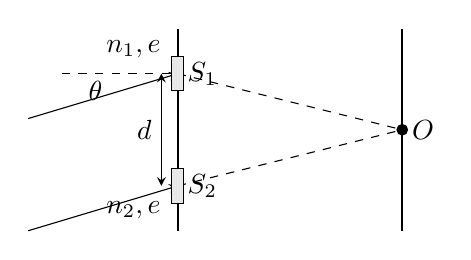
\begin{tikzpicture}[scale=0.95,>=stealth]
 \draw[thick] (0,-1.35) -- (0,1.35);
 \filldraw (0,0.75) circle (2pt) node[right] {\(S_1\)};
 \filldraw (0,-0.75) circle (2pt) node[right] {\(S_2\)};
 \draw[<->] (-0.22,-0.75) -- (-0.22,0.75) node[midway,left] {\(d\)};
 \draw[thick] (3.0,-1.35) -- (3.0,1.35);
 \filldraw (3.0,0) circle (2pt) node[right] {\(O\)};
 \draw[dashed] (0,0.75) -- (3.0,0);
 \draw[dashed] (0,-0.75) -- (3.0,0);
 \draw[->] (-2.0,0.15) -- (0,0.75);
 \draw[->] (-2.0,-1.35) -- (0,-0.75);
 \draw[dashed] (-1.55,0.75) -- (0,0.75);
 \node at (-1.1,0.52) {\(\theta\)};
 \draw[fill=gray!18] (-0.08,0.52) rectangle (0.08,0.98);
 \draw[fill=gray!18] (-0.08,-0.98) rectangle (0.08,-0.52);
 \node[left] at (-0.1,1.08) {\(n_1,e\)};
 \node[left] at (-0.1,-1.08) {\(n_2,e\)};
\end{tikzpicture}
\end{center}
\end{exercise}

\begin{solution}
中央 \(O\) 处的出射几何路程满足 \(S_1O=S_2O\)，所以相位差只来自两件事：斜入射时两缝处入射波本来就有相位差，以及两块介质片带来的附加光程差。

约定 \(\delta_{12}=L_1-L_2\)，即用通过 \(S_1\) 的光路减通过 \(S_2\) 的光路。介质片带来的光程差为 \(\delta_{\text{film}}=(n_1-n_2)e\)。
按原图的入射方向，波先到达上缝 \(S_1\)，后到达下缝 \(S_2\)。因此以 \(S_1\) 光路减 \(S_2\) 光路时，斜入射带来的入射端光程差为
 \(\delta_{\text{inc}}=-d\sin\theta,\qquad \delta_{12}=\delta_{\text{film}}+\delta_{\text{inc}} =(n_1-n_2)e-d\sin\theta,\qquad \Delta\phi_{12}=\frac{2\pi}{\lambda}\left[(n_1-n_2)e-d\sin\theta\right].\) 
总光程差和相位差就由上式给出。
若题目改成正入射，\(\theta=0\)，结果退化为两块介质片的相位差；若反过来定义“第二路减第一路”，整个相位差会整体变号，但明暗判据不变。
\end{solution}

\begin{theorem}[薄透镜的等光程性]
\begin{enumerate}
    \item 平行光经薄透镜后会汇聚到焦点。对称地看，凡是入射方向相同、出射到同一焦点的几条光线，薄透镜只改变它们的传播方向，不改变它们到焦点的总光程，所以它们在焦点处同相。
    \item 薄透镜可把近轴平行光汇聚于焦平面。因为透镜各部分对称，入射于透镜不同位置的平行光，经过透镜后到焦平面的总光程相等，故焦平面可看作等光程面。
    \item 物点 \(S\) 经薄透镜成像为 \(S'\) 时，从 \(S\) 出发、经透镜到 \(S'\) 的各条近轴光线，光程相等。
\end{enumerate}
\[
L_{AF}=L_{BF}=L_{CF}.
\]
\end{theorem}

\begin{exercise}[2011级期末：双缝装置浸入透明液体后的级次变化]
在杨氏双缝干涉实验中，设 \(SS_1=SS_2\)，用波长为 \(\lambda\) 的单色光照射双缝 \(S_1,S_2\)，通过空气后在屏 \(E\) 上形成干涉条纹。已知屏上某点 \(P\) 处为第三级明纹。若将整个装置放入某种透明液体中，\(P\) 点变为第四级明纹，求该液体的折射率 \(n\)。
\end{exercise}

\begin{solution}
整个装置浸入液体后，几何路程差 \(\Delta r\) 不变，改变的是光程差：同一段几何路程在液体中要乘上折射率 \(n\)。因此这题不是条纹间距简单缩放，而是同一个屏上点 \(P\) 对应的级次改变。空气中 \(P\) 为第三级明纹，说明 \(\Delta r=3\lambda\)。液体中光程差变为 \(\Delta L'=n\Delta r\)；若 \(P\) 变为第四级明纹，则
 \(n\Delta r=4\lambda,\qquad \Delta r=3\lambda \implies 3n\lambda=4\lambda \implies n=\frac43\approx 1.33.\) 
\end{solution}


\begin{exercise}[2007级期末：双缝明纹加高折射率反射面后变暗]
在双缝干涉实验中，屏幕 \(E\) 上 \(P\) 点原来是明条纹。若将缝 \(S_2\) 盖住，并在 \(S_1S_2\) 连线的垂直平分面处放一高折射率介质反射面 \(M\)，使 \(S_1\) 经反射面形成的虚像位置与原来的 \(S_2\) 等效。判断此时 \(P\) 点是明条纹还是暗条纹。

\begin{center}

\includegraphics[width=0.30\linewidth]{pdf-exercises/pdf2007-q07-lloyd-mirror.png}
\end{center}
\end{exercise}

\begin{solution}
反射面放在 \(S_1S_2\) 连线的垂直平分面处，反射光可看成来自 \(S_1\) 关于镜面的虚像，而这个虚像与原来的 \(S_2\) 等效。几何光程关系因此继承了原双缝中 \(S_1,S_2\) 到 \(P\) 的关系。

原来 \(P\) 为明纹，说明两缝到 \(P\) 的光程差满足 \(\Delta L=k\lambda\)。现在一路为 \(S_1\) 直达 \(P\)，另一路为 \(S_1\) 经高折射率反射面反射后到 \(P\)。由于反射等效虚源为 \(S_2\)，几何部分仍对应整数倍波长；但从空气侧在高折射率介质表面反射，会产生半波损失，相当于额外相差 \(\lambda/2\)。因此总光程差变为
 \(\Delta L'=k\lambda+\frac{\lambda}{2} =\left(k+\frac12\right)\lambda.\) 
所以 \(P\) 点变为暗条纹。本题不是说“盖住一个缝就没有干涉”；反射面提供了第二路相干光，真正改变明暗的是高折射率反射带来的半波损失。
\end{solution}
